\documentclass[main.tex]{subfile}

\begin{document}

\section{First Order Differential Equations}
\label{sec:foAnalysis}

\subsection{Background}
\label{sec:fo_analytical_view}

An example of a first order differential equation in circuitry can be derived
from the Butterworth filter circuit as shown in \figref{foCircuit}.

\begin{figure}[H]
	\begin{center}
		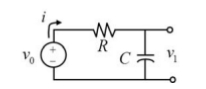
\includegraphics{foCircuit}
	\end{center}
	\caption{First Order Butterworth Filter (graphic taken from lab manual)}
	\label{fig:foCircuit}
\end{figure}

In analyzing the circuit we wish to find the voltage across the capacitor (this
can also be viewed as the output of the filter). First we apply the Kirchoff's
Voltage Law to the circuit:

\begin{align}
	V_0(t) &= V_R + V_C \label{eq:kvl}
	\\V_R &= iR \label{eq:ohmLaw}
	\\i &= C\frac{dV_C}{dt} \label{eq:capVoltage}
\end{align}
where $V_0$ is the voltage supply, $i$ is the current of the curcuit, $V_C$ is
the voltage across the capacitor, and $R$ and $C$ are the resistor and capacitor
values respectively. If we substitute \eqref{ohmLaw} and \eqref{capVoltage} into
\eqref{kvl} we get the following first order ODE:

\begin{align}
	RC\frac{dV_c}{dt} + V_c &= V_0(t) \label{eq:fo_ODE1}
\end{align}
If $V_0(t)$ is some step signal with magnitude voltage ($V_s$) then
\eqref{fo_ODE1} can be solved using the generic form (see equation $2.10$ in the
textbook):

\begin{align}
	V_C(t) = \left. V_s(1 - e^{\frac{-t}{\tau}}) \right| \tau = RC \label{eq:fo_Vc}
\end{align}
The constant $\tau$ is known as the time constant and has the property of.
$V_c(\tau) = (0.632)V_s$. Indeed we can see that the time constant $\tau$ has
units of time: 

	\[RC = (\frac{[M] * [L]^2}{[T]^2 * I^2} )(\frac{[T]^4 * [I]^2}{[M] * [L]^2}) = [T]\]

\subsection{Experimental Analysis}

The lab "experiment" was conducted using LabView. First, a signal generator
block was placed and configured to produce a 1Hz square wave. The generator
output was then connected to a filter block configured to simulate a first order
lowpass Butterworth filter with a cutoff frequency of 30 Hz. Finally, both the
output of the signal generator and the output of the filter were connected to a
graph block so both the original and filtered waves could be seen.

% subsection background (end)

\tabref{fo_a_taus} shows the theoretical resistor and capacitor values along
with their theoretical time constant values and their corresponding experimental
contants. As seen the percent-error in for both time constant values are less
than $10\%$ - which, simply stated, means that the \Labview model and our
mathematical model agree with eachother. Assuming the theoretical model is an
accurate representation of the system we find then that \Labview is a good
enough simulator for modeling realworld first order ODE systems. One must note
however that if the frequency of the wave generator is to high (smaller than the
system's time constant) then the system will never settle to it's steady state
value, and possibly not even reach the proper rise time.

\begin{table}[H]
  \begin{center}
		\caption{Analytical Time Constants}
		\label{tab:fo_a_taus}
		\begin{tabular}{ccccc}
      \\ \toprule
			\\ $R$ ($\Omega$) & $C$ (\dem{mF}) & $\tau_{\text{th}} = RC$ (\dem{s}) & $\tau_{\text{exp}} = RC$ (\dem{s}) & $\%Error$
      \\ \midrule
			\\  100 &  0.1061 &  1.061e-02 &  1.011e-02 &  -4.74
 \\  50 &  0.1061 &  5.305e-03 &  4.811e-03 &  -9.32
      \\ \bottomrule
    \end{tabular}
  \end{center}
\end{table}

\begin{figure}[H]
	\begin{center}
    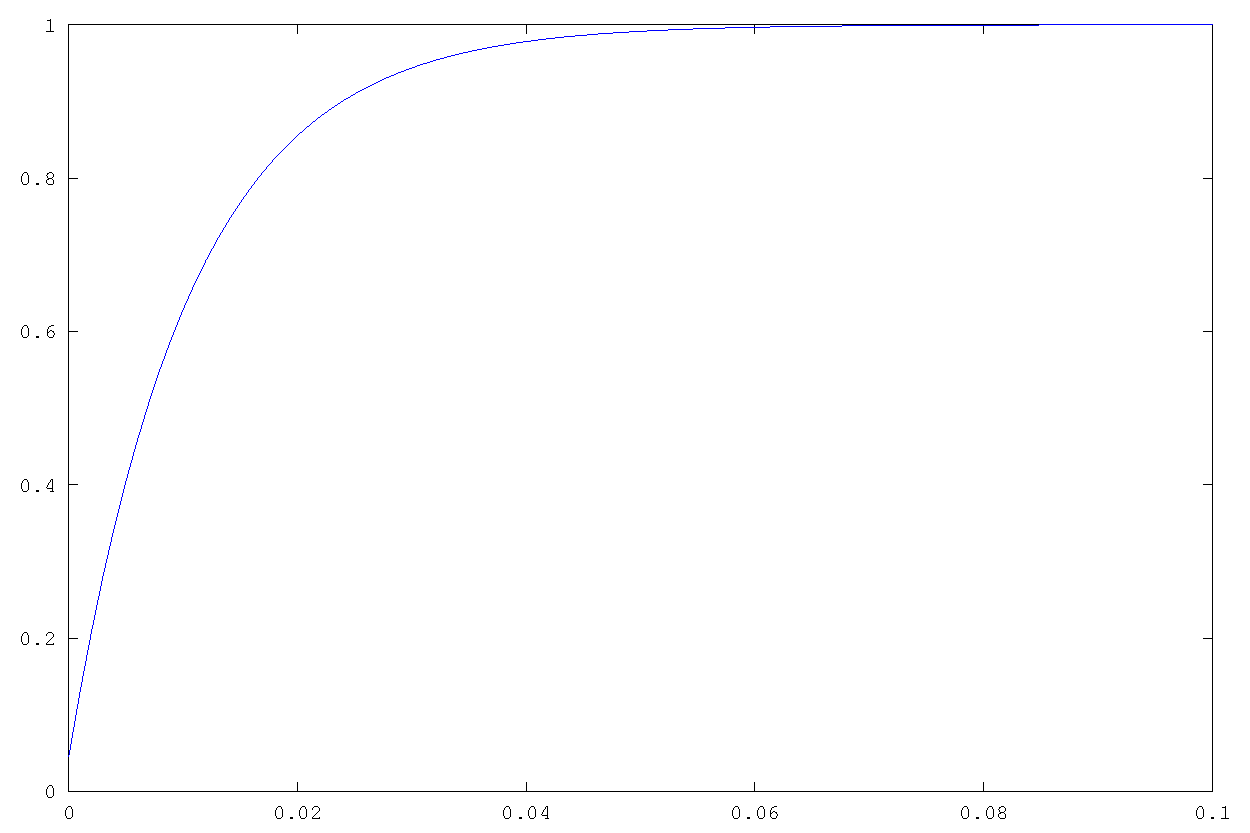
\includegraphics[width=\linewidth]{foAnalResponse1.pdf}
	\end{center}
	\caption{First Order Butterworth Response}
	\label{fig:foGraph}
\end{figure}

% section analytical_time_constants (end)

% section first_order_differential_equations (end)

\end{document}
